\section{LLM-only vs.\ KG-grounded evaluation}\label{sec:eval}

\subsection{Setup}
Ten competency questions were selected to include multi-hop (CQ4, CQ5, CQ8, CQ10, CQ11, CQ13) and
inference-dependent questions (CQ2, CQ6, CQ8, CQ13). Each was asked in two conditions with the same model
(\evalModel{} on Groq), temperature~0 and the same token limit: (A) the LLM alone with a short system prompt
stating the snapshot date, and (B) the LLM with retrieved graph facts (Section~\ref{sec:app}). Expected answers
were verified against the official IPL points table (CQ1--CQ3) or against ground truth recomputed from the
cleaned match table. A keyword check gave a first pass; every verdict was then reviewed by hand
(\texttt{scripts/run\_cq\_evaluation.py}, \texttt{Results/iteration2/cq\_evaluation\_review.csv}).

{\footnotesize
\begin{longtable}{p{2.5cm}p{2.8cm}p{3.3cm}p{3.3cm}p{1.0cm}p{1.0cm}}
\caption{LLM-only (A) vs KG-grounded (B) answers on 10 competency questions (openai/gpt-oss-120b, temperature 0, identical settings). Answers summarised; full text in Appendix~\ref{app:answers}.}\label{tab:cq-eval}\\
\toprule \textbf{CQ / question} & \textbf{Expected answer} & \textbf{LLM only (A)} & \textbf{KG-grounded (B)} & \textbf{Correct? A/B} & \textbf{Evidence? A/B} \\ \midrule \endfirsthead
\toprule \textbf{CQ / question} & \textbf{Expected answer} & \textbf{LLM only (A)} & \textbf{KG-grounded (B)} & \textbf{Correct? A/B} & \textbf{Evidence? A/B} \\ \midrule \endhead
\bottomrule \endfoot
\textbf{CQ1}: How many points do Punjab Kings have after match 39 of IPL 2026, and what is their won / lost / no-result record? & 13 points from 7 matches: 6 won, 0 lost, 1 no result. & Claims 10 points and a 5-4-0 record from 9 matches; actual 13 points, 6-0-1 from 7. & Correct (13 points, 6 won, 0 lost, 1 no result). The automatic keyword check missed the plural '6 wins'. & No / Yes & No / Yes \\ \midrule
\textbf{CQ2}: Which four teams hold the qualifying places in IPL 2026 after match 39, and how are SRH and RR separated? & PBKS 13, RCB 12, SRH 10, RR 10. SRH and RR are level on 10 points and on wins (5 each, tie-break 1), so net run rate decides (tie-break 2): SRH 0.815 v RR 0.602. & Names MI, CSK, KKR, SRH as the top four with invented points and NRR values; only SRH is right. & Correct top four; applies tie-break 1 (wins, both 5) then tie-break 2 (NRR 0.815 v 0.602). & No / Yes & No / Yes \\ \midrule
\textbf{CQ3}: What is Kolkata Knight Riders' net run rate after match 39 of IPL 2026? & -0.751 (the source points table shows +0.751, a dropped minus sign). & Invents +0.212 and a 4-4 record; actual -0.751. & Correct (-0.751), taken from the rule-derived standing. & No / Yes & No / Yes \\ \midrule
\textbf{CQ4}: Which fixtures does Rajasthan Royals still have to play after match 39 of IPL 2026? & 6 fixtures: PBKS (match 40, Mullanpur), DC (match 43, Jaipur), GT (match 52, Jaipur), DC (match 62, New Delhi), LSG (match 64, Jaipur), MI (match 69, Mumbai). & Lists 7 fixtures (SRH, KKR, MI, CSK, DC, GT, RCB) with invented dates and venues; actual 6. & Correct: all 6 fixtures with match numbers, dates and venues. & No / Yes & No / Yes \\ \midrule
\textbf{CQ5}: What is the highest points total Lucknow Super Giants can still reach in IPL 2026 if they win all their remaining matches? & 16 points: 4 now plus 6 remaining matches x 2. & Assumes 6 points and 7 matches left, giving 20; actual 4 points, 6 left, maximum 16. & Correct (16 = 4 + 6 x 2), citing rule R3. & No / Yes & No / Yes \\ \midrule
\textbf{CQ6}: Which teams are mathematically eliminated from the IPL 2026 top 4 after match 39? & None. Even last-placed LSG can reach 16 points while the leader has 13, so every team is still in contention. & Claims PBKS and RR are eliminated on 2 points - the opposite of the truth (PBKS lead the table). & Correct: no team eliminated, with the reason (lowest maximum 16 \textgreater{} leader's 13). & No / Yes & No / Yes \\ \midrule
\textbf{CQ8}: Which of Rajasthan Royals' remaining opponents are direct rivals still in contention for the top 4 in IPL 2026? & All six remaining opponents are still in contention: GT (8 pts, closest), PBKS (13), DC (6, twice), LSG (4), MI (4). & Names KKR, SRH, GT; KKR and SRH are not remaining opponents and all points are invented. & Correct: all six remaining opponents, ordered by points gap. & No / Yes & No / Yes \\ \midrule
\textbf{CQ10}: If Kolkata Knight Riders lose their last league match of IPL 2026, which teams are certain to finish above them on points? & Scenario: KKR's last match is match 70 v DC; KKR could then reach at most 15 points. No team is certain to finish above; all nine others could still finish level or above. & Says four teams (SRH, RCB, DC, MI) are certain to finish above; actual none; points invented. & Correct: presented as a scenario; no team certain above; KKR capped at 15. & No / Yes & No / Yes \\ \midrule
\textbf{CQ11}: Which teams has Rajasthan Royals beaten in IPL 2026 so far, and at which venues? & CSK (match 3, Guwahati), GT (match 9, Ahmedabad), MI (match 13, Guwahati), RCB (match 16, Guwahati), LSG (match 32, Lucknow). & Lists 4 wins (MI, SRH, KKR, RCB); RR actually lost to SRH and KKR and has 5 wins. & Correct: all 5 wins with venues. & No / Yes & No / Yes \\ \midrule
\textbf{CQ13}: At which venues has Rajasthan Royals played in IPL 2026 so far? & 6 venues: Barsapara Cricket Stadium (Guwahati), Ekana Cricket Stadium (Lucknow), Eden Gardens (Kolkata), Narendra Modi Stadium (Ahmedabad), Rajiv Gandhi International Stadium (Hyderabad), Sawai Mansingh Stadium (Jaipur). & Lists 7 venues incl. Wankhede, DY Patil, Chinnaswamy; RR had not played at these by match 39. & Correct: all 6 venues (inferred playedAtVenue chain). & No / Yes & No / Yes \\ \midrule
\end{longtable}}


\begin{figure}[H]\centering
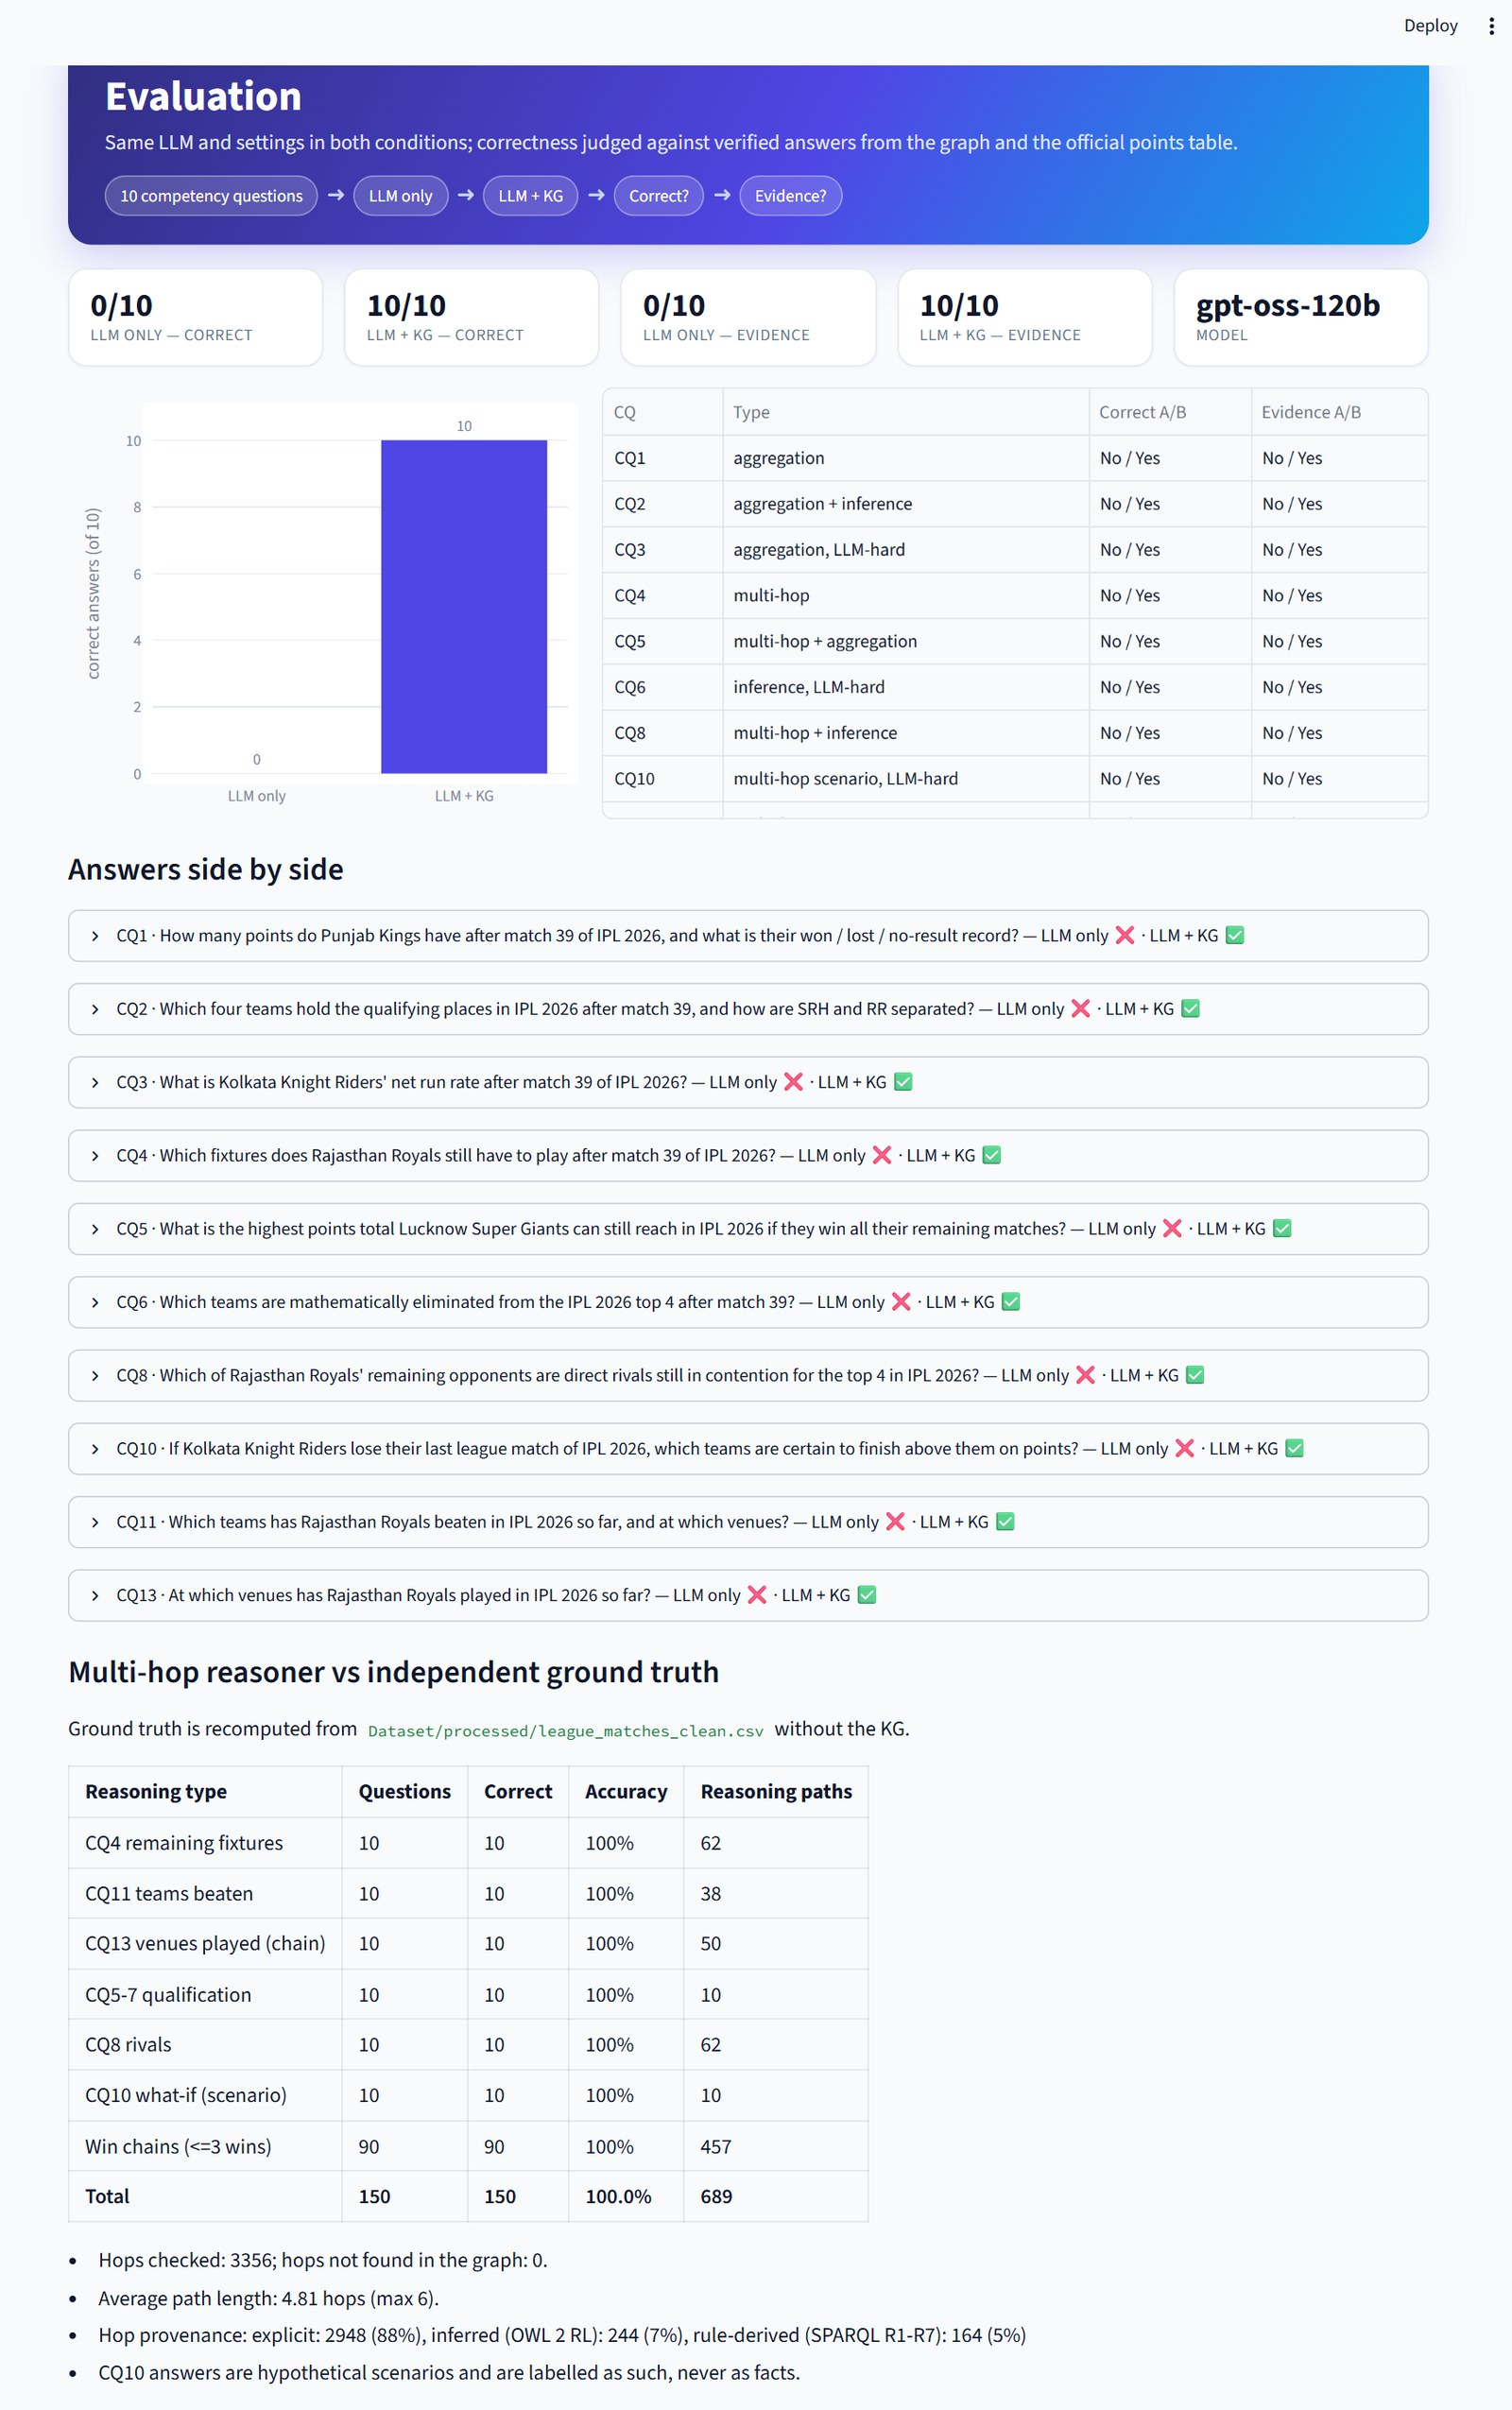
\includegraphics[width=0.92\linewidth]{figures/app_evaluation.jpg}
\caption{Evaluation page of the application.}
\end{figure}

\subsection{Results}
\begin{itemize}
  \item \textbf{Correctness:} LLM only \evalA/10; KG-grounded \evalB/10.
  \item \textbf{Evidence available:} LLM only 0/10; KG-grounded \evidB/10 --- every grounded answer cites the
        retrieved facts it used.
  \item \textbf{Unsupported or hallucinated claims:} all ten LLM-only answers contained invented specifics
        (points, records, fixtures, venues, NRR values), stated confidently; it never said it did not know. No
        grounded answer contained a claim outside the retrieved facts.
  \item \textbf{Where grounding helped most:} questions whose answers exist only in this season's data (CQ1,
        CQ3, CQ4), and inference-dependent questions, where the LLM-only answer was not just inaccurate but
        reversed --- for CQ6 it declared the table leaders PBKS eliminated.
  \item \textbf{Where grounding did not help:} grounding cannot add knowledge the graph lacks. Questions about
        players (top run scorer) are correctly refused rather than answered. Grounding also leaves phrasing to
        the LLM: for CQ10 the grounded answer is correct but omits the opponent of KKR's last match, which was
        in the retrieved facts.
\end{itemize}
The LLM-only failures are not a weakness of this particular model: IPL~2026 happened after its training data,
so without retrieval any LLM can only guess. That is exactly the gap the knowledge graph fills.
